% !TEX root = base-r.tex

\begin{seeblock}{Strings}{stringr}
  \small\renewcommand{\arraystretch}{1.5}
  \begin{tabular}{c >{\footnotesize} p{0.45\linewidth}}
    \inline{paste(x, y, sep = ' ')} & Join multiple vectors together.\\
    \inline{paste(x, collapse = ' ')} & Join elements of a vector together.\\
    \inline{grep(pattern, x)} & Find regular expression matches in \inl{x}.\\
    \inline{gsub(pattern, replace, x)} & Replace matches in \inl{x} with a string.\\
    \inline{toupper(x)} & Convert to uppercase.\\
    \inline{tolower(x)} & Convert to lowercase.\\
    \inline{nchar(x)} & Number of characters in a string.
%    \inl{sprintf(fmt, ...)} & Return a character vector containing a formatted combination of text and variable values.
  \end{tabular}
\end{seeblock}

\begin{block}{Factors}
  \begin{columns}[t]\hfill
    \begin{column}{.45\linewidth}\centering
      \inline{factor(x)}\\Turn a vector into a factor. Can set the levels of the factor and the order.
    \end{column}
    \begin{column}{.45\linewidth}\centering
      \inline{cut(x, breaks = 4)}\\Turn a numeric vector into a factor by 'cutting' into sections.
    \end{column}\hfill
  \end{columns}
\end{block}

{\setbeamercolor{block body}{fg = black, bg = white}
\begin{block}{Statistics}
  \begin{columns}\hfill\small
    \begin{column}{.45\linewidth}\centering
      \begin{tikzpicture}[remember picture, overlay]
        \draw[darkgray, dotted, very thick, rounded corners] (-0.45, .25) rectangle (3.35, -2.45);
      \end{tikzpicture}
      \inline{lm(y~x, data=df)}\\Linear model.\\[1ex]
      \inline{glm(y~x, data=df)}\\Generalized linear model.\\[1ex]
      \inline{summary}\\Get more detailed information out a model.
    \end{column}\hspace{-2ex}
    \begin{column}{.3\linewidth}\centering
      \inline{t.test(x, y)}\\Perform a t-test for difference between means.\\[1ex]
      \inline{pairwise.t.test}\\Perform a t-test for paired data.
    \end{column}\hspace{-2ex}
    \begin{column}{.225\linewidth}\centering
      \inline{prop.test}\\Test for a difference between proportions.\\[1ex]
      \inline{aov}\\Analysis of variance.
    \end{column}\hfill
  \end{columns}
\end{block}

\begin{block}{Distributions}\small
  \renewcommand{\arraystretch}{1.5}
  \begin{tableau}{| >{\color{black}} c | *{2}{>{\color{black}\centering}m{0.15\linewidth} |} >{\color{black}\centering}m{0.2\linewidth} | >{\color{black}} c |}
    \cline{2-5}
    \multicolumn{1}{l|}{} & Random Variates & Density Function & Cumulative Distribution& Quantile\\\hline
    \rowcolor{secondary} Normal & \inline{rnorm} & \inline{dnorm} & \inline{pnorm} & \inline{qnorm}\\\hline
    Poisson & \inline{rpois} & \inline{dpois} & \inline{ppois} & \inline{qpois}\\\hline
    \rowcolor{secondary} Binomial & \inline{rbinom} & \inline{dbinom} & \inline{pbinom} & \inline{qbinom}\\\hline
    Uniform & \inline{runif} & \inline{dunif} & \inline{punif} & \inline{qunif}\\\hline
  \end{tableau}
\end{block}
}

\begin{seeblock}{Plotting}{ggplot2}
  \vspace{1ex}
  \begin{columns}\hfill
    \begin{column}{.05\linewidth}\centering
      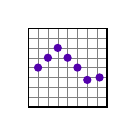
\begin{tikzpicture}[scale = 0.125]
        \fill[white] (0, 0) rectangle (8, 8);
        \draw[step = 1, ultra thin, gray] (0, 0) grid (8, 8);
        
        \foreach \x/\y in {1/4, 2/5, 3/6, 4/5, 5/4, 6/2.75, 7.25/3}
          \fill[violet!65!blue] (\x, \y) circle (12pt);
        \draw (0, 0) rectangle (8, 8);
      \end{tikzpicture}
    \end{column}\hspace{0.1ex}
    \begin{column}{.2\linewidth}\centering
      \inline{plot(x)}\\Values of x in order.
    \end{column}\hspace{-2ex}
    \begin{column}{.05\linewidth}\centering
      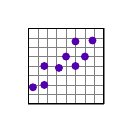
\begin{tikzpicture}[scale = 0.12]
        \fill[white] (0, 0) rectangle (8, 8);
        \draw[step = 1, ultra thin, gray] (0, 0) grid (8, 8);
        
        \foreach \x/\y in {0.5/1.75, 1.7/2, 1.7/4, 3.25/3.8, 4/5, 5/4, 5/6.6, 6/5, 6.8/6.7}
          \fill[violet!65!blue] (\x, \y) circle (12pt);
        \draw (0, 0) rectangle (8, 8);
      \end{tikzpicture}
    \end{column}
    \begin{column}{.25\linewidth}\centering
      \inline{plot(x, y)}\\Values of x against y.
    \end{column}\hspace{-2ex}
    \begin{column}{.05\linewidth}\centering
      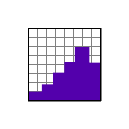
\begin{tikzpicture}[scale = 0.115]
        \fill[white] (0, 0) rectangle (8, 8);
        \draw[step = 1, ultra thin, gray] (0, 0) grid (8, 8);
        
        \fill[violet!65!blue] (0, 0) -- (0, 1) -- (1.5, 1) -- (1.5, 1.8) -- (2.75, 1.8) -- (2.75, 3.1) -- (4, 3.1) -- (4, 4.25) -- (5.15, 4.25) -- (5.15, 5.9) -- (6.75, 5.9) -- (6.75, 4.2) -- (8, 4.2) -- (8, 0) -- cycle;
        
        \draw (0, 0) rectangle (8, 8);
      \end{tikzpicture}
    \end{column}
    \begin{column}{.2\linewidth}\centering
      \inline{hist(x)}\\Histogram of x.
    \end{column}\hfill
  \end{columns}
\end{seeblock}

\begin{annotedblock}{Dates}{See the \textbf{lubridate} package.}
\end{annotedblock}
